\chapter{CARE Survey Instrument}
\label{app:care-survey}

\newcommand{\ratingTable}{
    \vspace{0.5em}
    \begin{center}
\begin{tabular}{c c c c c c}
    $\bigcirc$ & $\bigcirc$ & $\bigcirc$ & $\bigcirc$ & $\bigcirc$ & $\bigcirc$ \\
    
    {\small \hspace{1em} Poor \hspace{1em}} & 
    {\small \hspace{1em} Fair \hspace{1em}} &
    {\small \hspace{1em} Good \hspace{1em}} & 
    {\small \hspace{1em} Very Good \hspace{1em}} &
    {\small \hspace{1em} Excellent  \hspace{1em}} &
    {\small \hspace{1em} Does Not Apply \hspace{1em}} \\ 
\end{tabular}
\end{center}
    \vspace{1em}
}

\begin{small}

\begin{tcolorbox}[boxrule=1pt]
    \begin{center}
         {\large \textbf{How was \sysname at ...}}
    \end{center}
   
\end{tcolorbox}

\vspace{1em}


% Question 1
\noindent \textbf{1. Making you feel at ease...} \\
\textit{(being friendly and warm towards you, treating you with respect; not cold or abrupt)}
\ratingTable

% Question 2
\noindent \textbf{2. Letting you tell your ``story''...} \\
\textit{(giving you time to fully describe your illness in your own words; not interrupting or diverting you)}
\ratingTable

% Question 3
\noindent \textbf{3. Really listening...} \\
\textit{(paying close attention to what you were saying)}
\ratingTable

% Question 4
\noindent \textbf{4. Being interested in you as a whole person...} \\ 
\textit{(asking/knowing relevant details about your life, your situation, not treating you as ``just a number'')}
\ratingTable


% Question 5
\noindent \textbf{5. Fully understanding your concerns...} \\
\textit{(communicating that your concerns were accurately understood; not overlooking or dismissing anything)}
\ratingTable

% Question 6
\noindent \textbf{6. Showing care and compassion...} \\
\textit{(seeming genuinely concerned, connecting with you on a human level; not being indifferent or ``detached'')}
\ratingTable

% Question 7
\noindent \textbf{7. Being Positive...} \\
\textit{(having a positive approach and a positive attitude; being honest but not negative about your problems)}
\ratingTable

% Question 8
\noindent \textbf{8. Explaining things clearly...} \\
\textit{(fully answering your questions, explaining clearly, giving you adequate information, not being vague)}
\ratingTable

% Question 9
\noindent \textbf{9. Helping you take control...} \\
\textit{(exploring with you what you can to to improve your health yourself; encouraging rather than ``lecturing'' you)}
\ratingTable

% Question 10
\noindent \textbf{10. Making a plan of action with you...} \\
\textit{(discussing the options, involving you in decisions as much as you want to be involved; not ignoring your views)}
\ratingTable
\end{small}

\section{Results from the CARE survey}
\label{appendix:CAREdist}

\Cref{fig:caredist} illustrates our feasibility study's distribution of CARE scores and compares it with the older \oldsysname \citep{brown2023mi}. The distribution for fully-generative \sysnamewithv is right-skewed, with the majority of participants assigning scores in the upper ranges (36–50). These results indicated that \sysname was more effective in promoting an empathetic interaction. However, the comparison in \cref{subsec:care} contextualized its performance relative to human counsellors as falling short of fully matching human-level empathy.

\Cref{fig:caremean} illustrates the mean scores of each question from the CARE survey across the 106 participants who interacted with \sysnamewithv, and compares it with that of \oldsysname. The fully-generative \sysnamewithv scores higher on each question. The most notable improvement seems to be for the question ``How was \sysname at showing care and compassion?''
Interestingly, the lowest-scoring question was ``How was \sysname at making a plan of action with you?'', despite the counsellor prompt directly instructing it to do so.


\begin{figure}[H]
\centering
  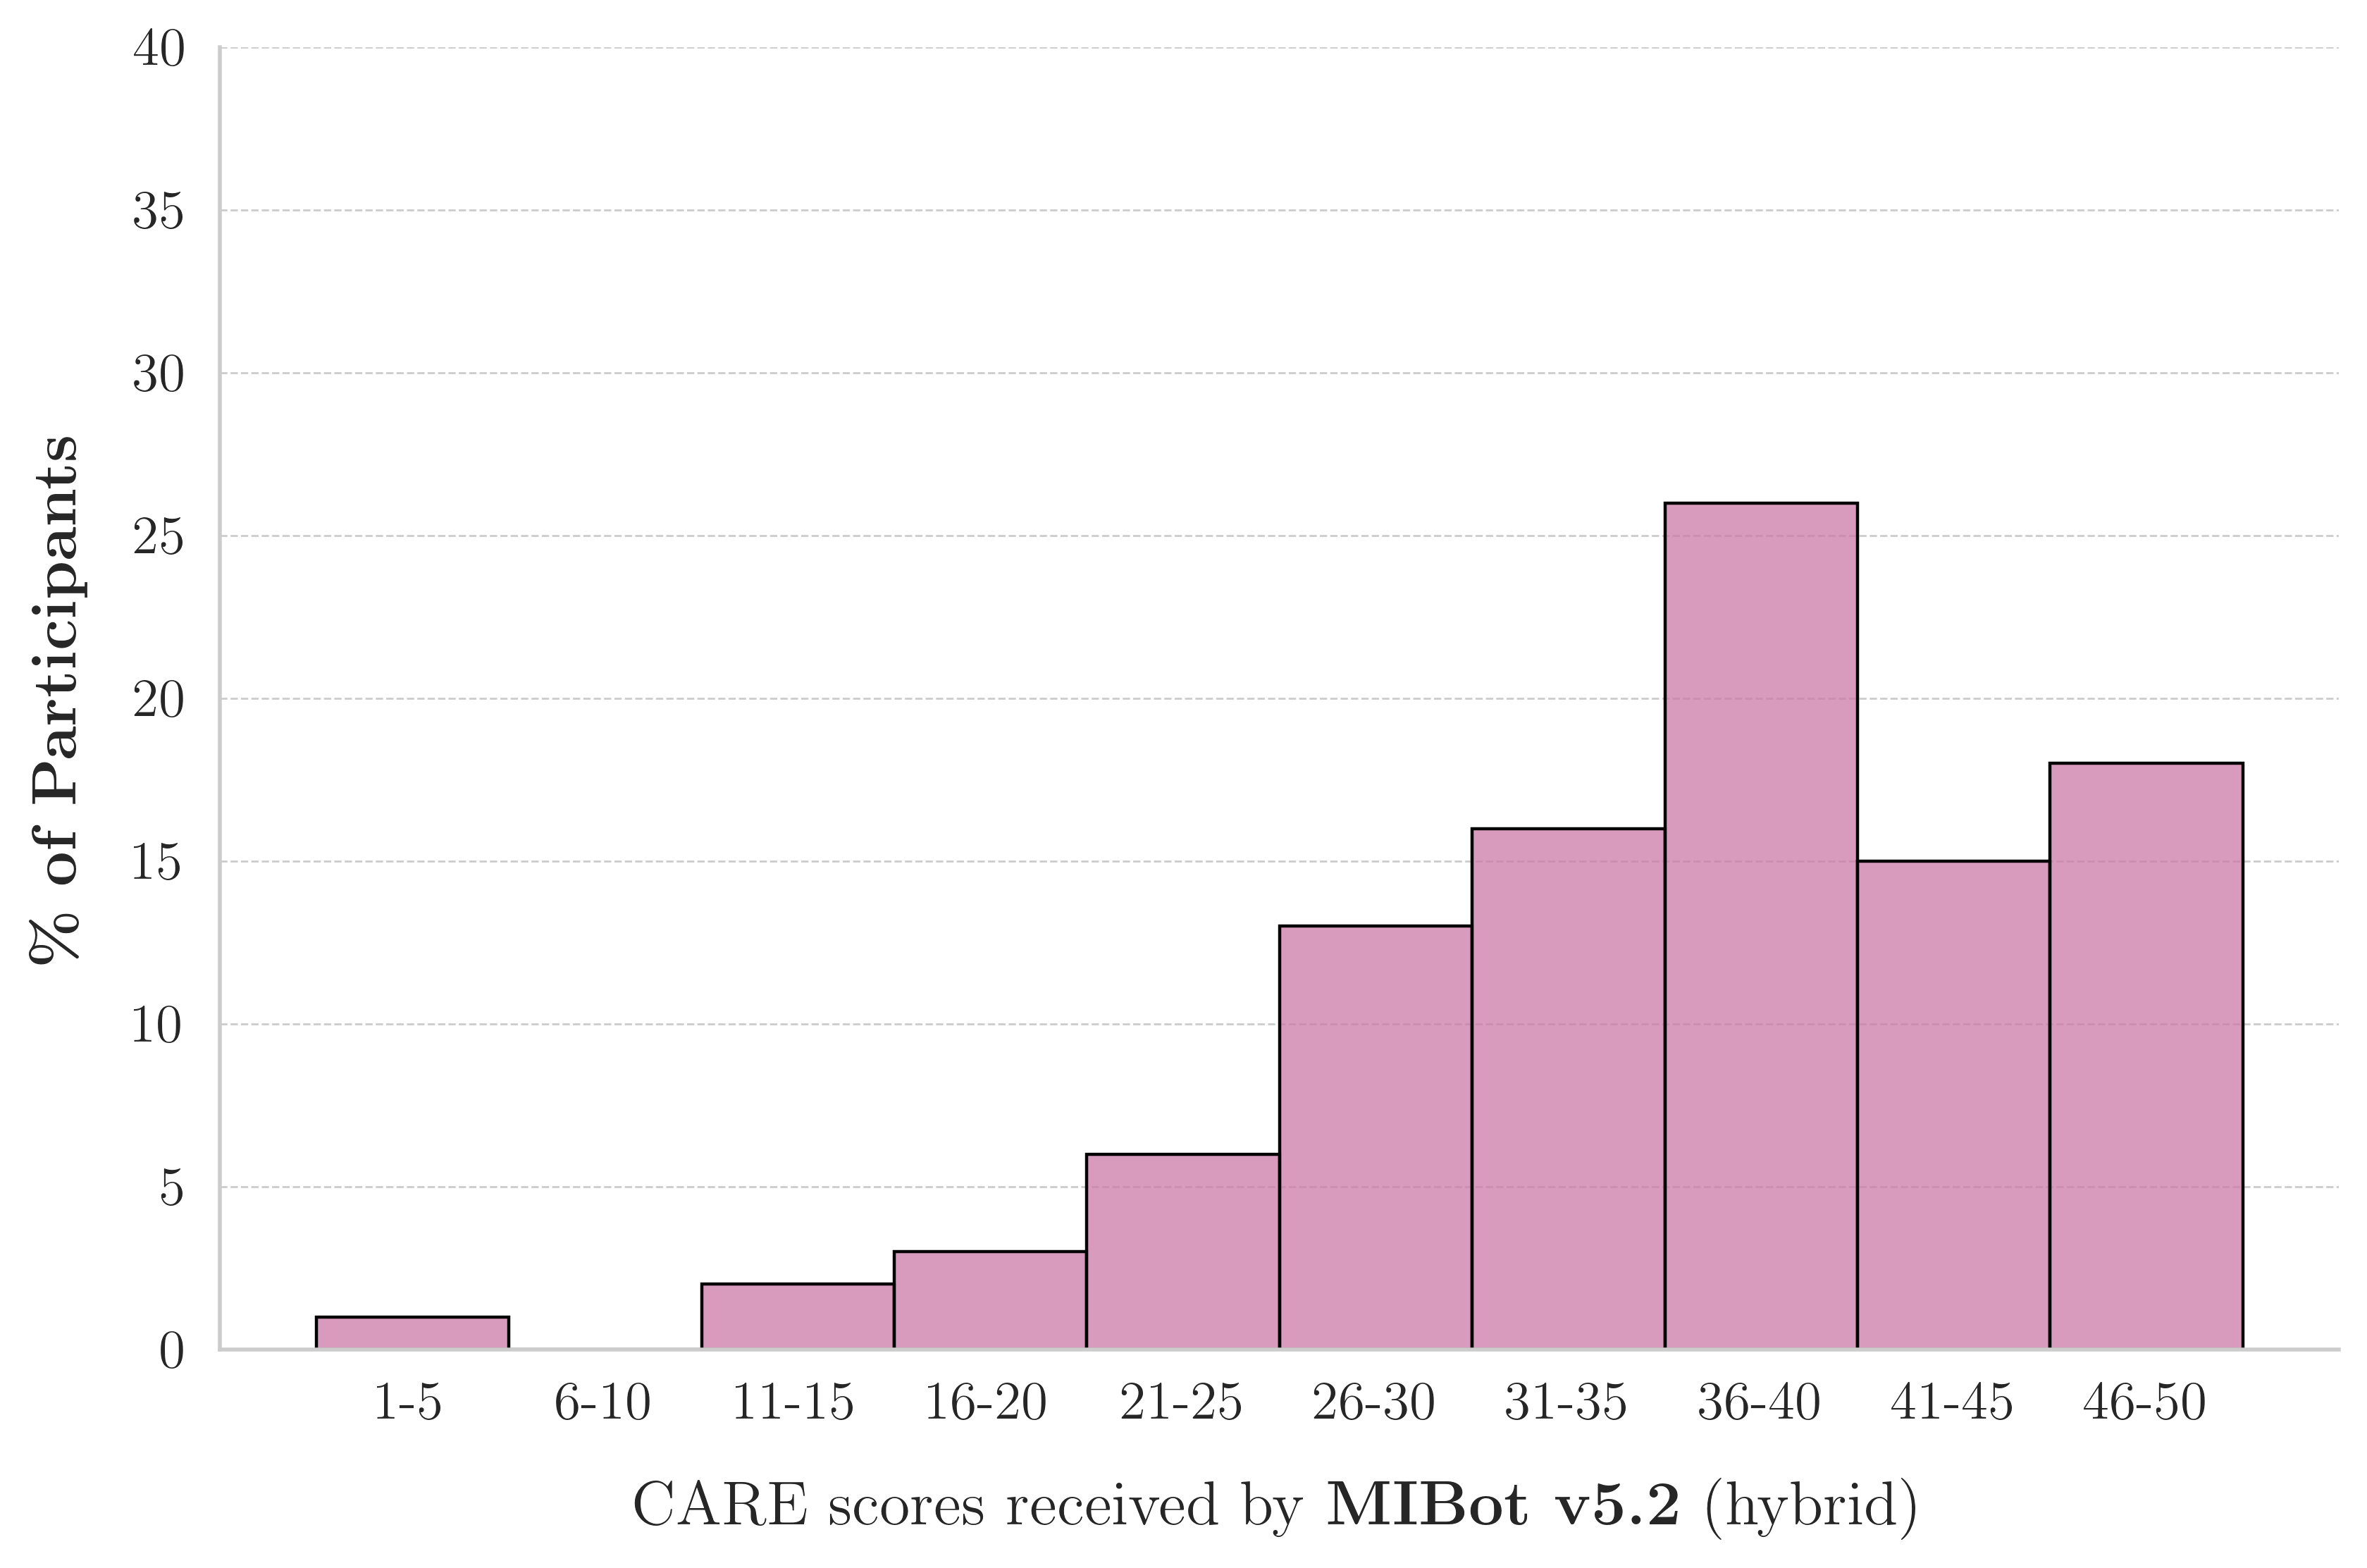
\includegraphics[width=0.48\textwidth]{fig/MIV5.2_care_scores_histogram.png} \hfill
  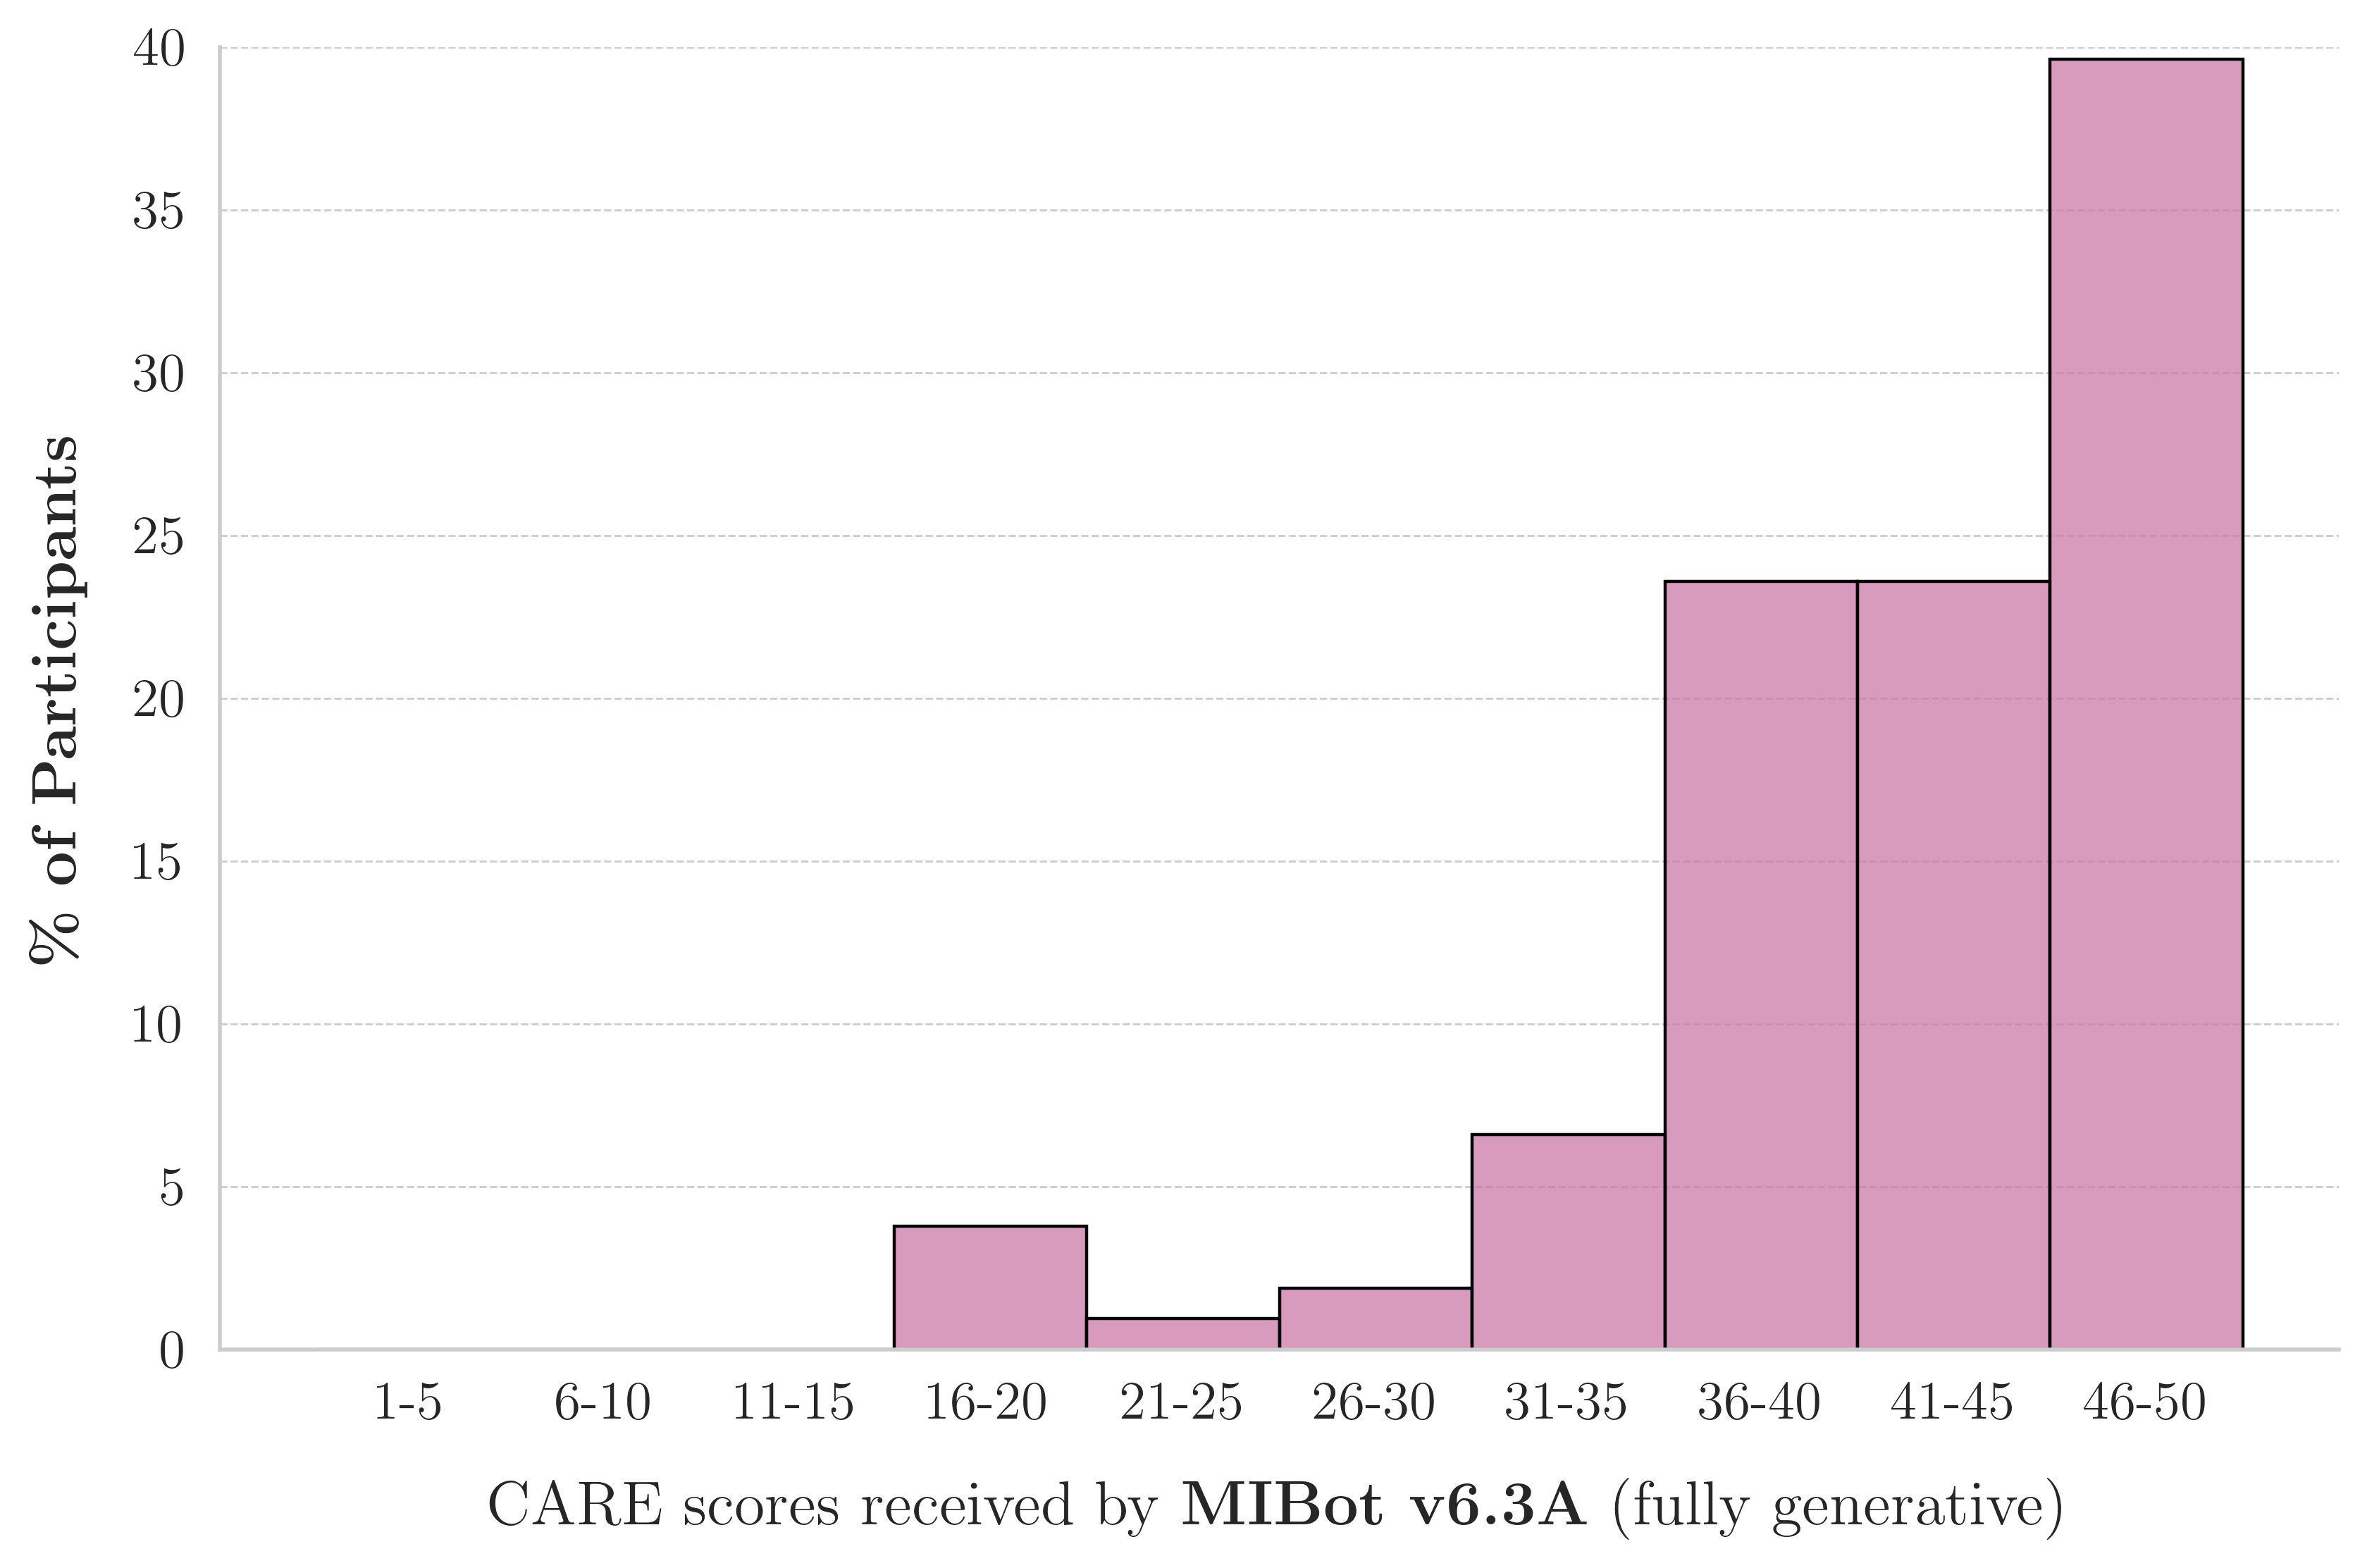
\includegraphics[width=0.48\textwidth]{fig/2024-11-14-MIV6.3A-2024-11-22-MIV6.3A_care_scores_histogram.png}
  \caption {Distribution of CARE scores for \oldsysname (hybrid) and \sysnamewithv (fully generative).}
  \label{fig:caredist}
\end{figure}



\vspace{-0.5cm}

\begin{figure}[!htbp]
\centering
  \includegraphics[width=0.8\textwidth]{fig/combined_care_scores_sorted_acl.png}
  \caption {Question-wise mean CARE scores for \oldsysname (hybrid) and \sysnamewithv (fully generative).}
  \label{fig:caremean}
\end{figure}
